\documentclass[border=10pt]{standalone}
\usepackage{tikz}
\usetikzlibrary{positioning, arrows.meta, calc, fit, backgrounds, decorations.pathreplacing}

\begin{document}
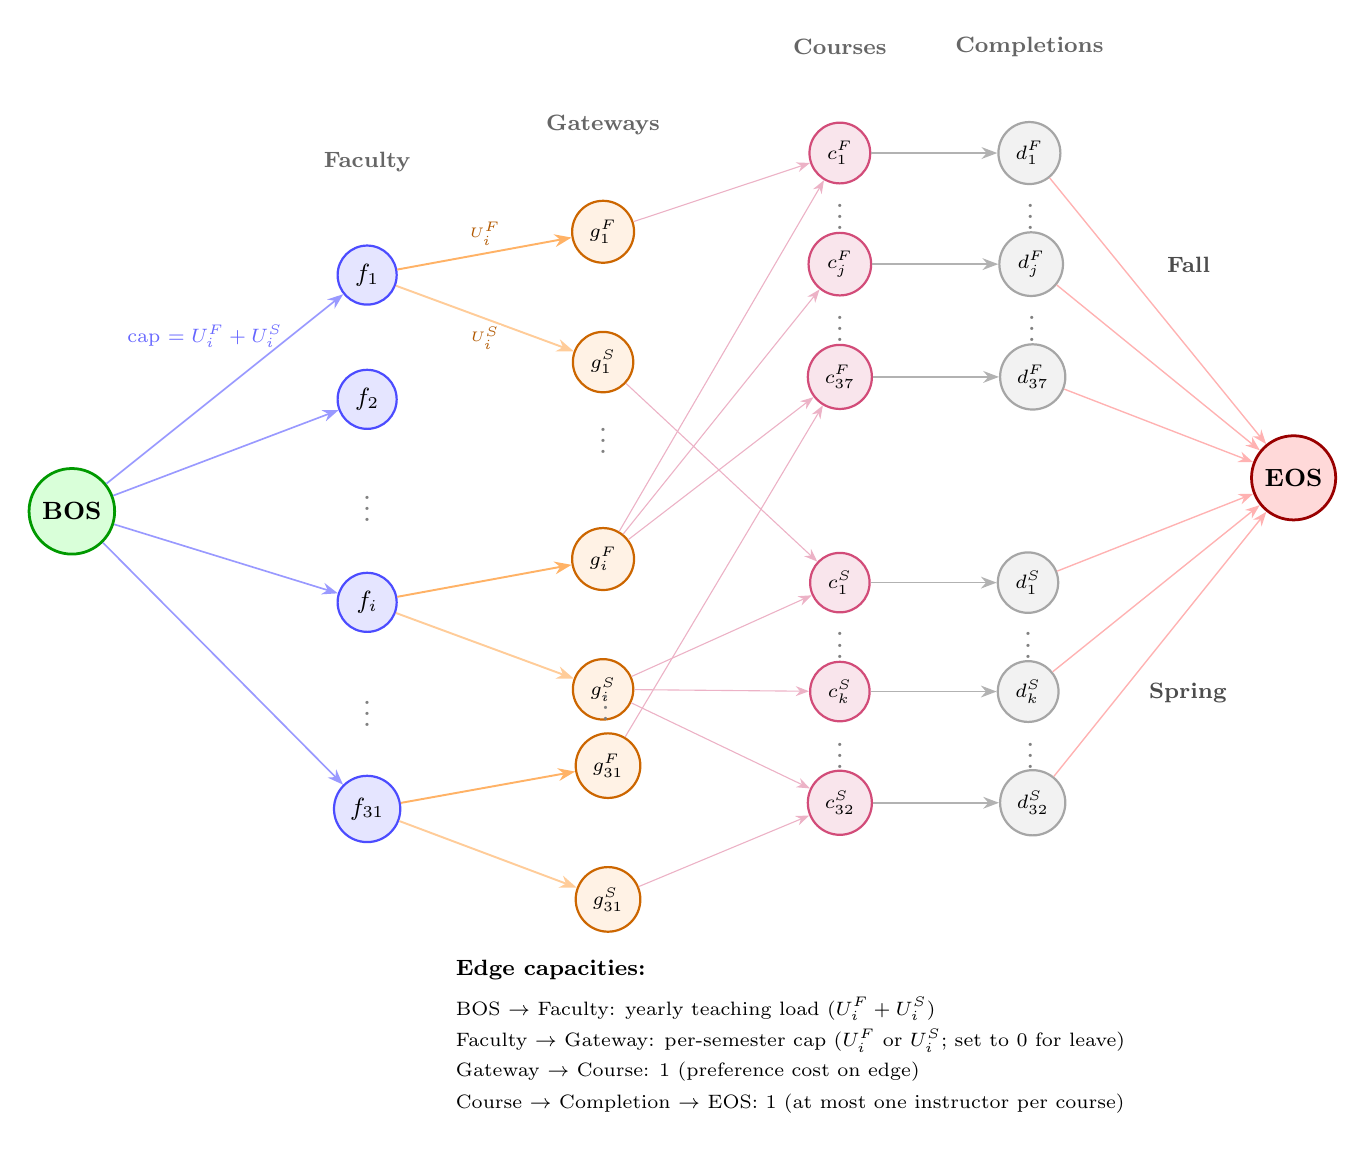
\begin{tikzpicture}[
    >=Stealth,
    node distance=1.8cm and 2.8cm,
    every node/.style={font=\small},
    bos/.style={circle, draw=green!60!black, fill=green!15, minimum size=0.9cm, line width=1pt, font=\small\bfseries},
    eos/.style={circle, draw=red!60!black, fill=red!15, minimum size=0.9cm, line width=1pt, font=\small\bfseries},
    faculty/.style={circle, draw=blue!70, fill=blue!10, minimum size=0.75cm, line width=0.8pt},
    gateway/.style={circle, draw=orange!80!black, fill=orange!10, minimum size=0.6cm, line width=0.8pt, font=\scriptsize},
    course/.style={circle, draw=purple!70, fill=purple!10, minimum size=0.6cm, line width=0.8pt, font=\scriptsize},
    completion/.style={circle, draw=gray!70, fill=gray!10, minimum size=0.5cm, line width=0.8pt, font=\scriptsize},
    edgelabel/.style={font=\scriptsize, midway, fill=white, inner sep=1pt},
    dots/.style={font=\large, text=gray},
    brancelabel/.style={font=\footnotesize\bfseries, text=black!70},
    layerlabel/.style={font=\footnotesize\bfseries, text=black!60},
]

% === BOS ===
\node[bos] (bos) {BOS};

% === Faculty nodes (spread out more vertically) ===
\node[faculty] (f1) [right=2.8cm of bos, yshift=3.0cm] {$f_1$};
\node[faculty] (f2) [below=0.8cm of f1] {$f_2$};
\node[faculty] (fi) [below=1.8cm of f2] {$f_i$};
\node[faculty] (fn) [below=1.8cm of fi] {$f_{31}$};

% dots between f2 and fi
\node[dots] at ($(f2)!0.5!(fi)$) {$\vdots$};
% dots between fi and fn
\node[dots] at ($(fi)!0.5!(fn)$) {$\vdots$};

% === Gateway nodes (more vertical separation between fall/spring pairs) ===
% Fall gateways
\node[gateway] (gf1) [right=2.2cm of f1, yshift=0.55cm] {$g^F_1$};
\node[gateway] (gfi) [right=2.2cm of fi, yshift=0.55cm] {$g^F_i$};
\node[gateway] (gfn) [right=2.2cm of fn, yshift=0.55cm] {$g^F_{31}$};

% Spring gateways (enough space so subscripts don't collide)
\node[gateway] (gs1) [below=0.85cm of gf1] {$g^S_1$};
\node[gateway] (gsi) [below=0.85cm of gfi] {$g^S_i$};
\node[gateway] (gsn) [below=0.85cm of gfn] {$g^S_{31}$};

% dots between gateway pairs
\node[dots] at ($(gs1)!0.5!(gfi) + (0, 0.35)$) {$\vdots$};
\node[dots] at ($(gsi)!0.5!(gfn) + (0, 0.35)$) {$\vdots$};

% === Course nodes (more vertical spread, clear separation between fall and spring groups) ===
% Fall courses (upper group)
\node[course] (cf1) [right=2.2cm of gf1, yshift=1.0cm] {$c^F_1$};
\node[course] (cfj) [below=0.6cm of cf1] {$c^F_j$};
\node[course] (cf37) [below=0.6cm of cfj] {$c^F_{37}$};
\node[dots] at ($(cf1)!0.5!(cfj)$) {$\vdots$};
\node[dots] at ($(cfj)!0.5!(cf37)$) {$\vdots$};

% Spring courses (lower group — clear gap from fall courses)
\node[course] (cs1) [below=1.8cm of cf37] {$c^S_1$};
\node[course] (csk) [below=0.6cm of cs1] {$c^S_k$};
\node[course] (cs32) [below=0.6cm of csk] {$c^S_{32}$};
\node[dots] at ($(cs1)!0.5!(csk)$) {$\vdots$};
\node[dots] at ($(csk)!0.5!(cs32)$) {$\vdots$};

% === Completion nodes ===
\node[completion] (df1) [right=1.6cm of cf1] {$d^F_1$};
\node[completion] (dfj) [right=1.6cm of cfj] {$d^F_j$};
\node[completion] (df37) [right=1.6cm of cf37] {$d^F_{37}$};
\node[dots] at ($(df1)!0.5!(dfj)$) {$\vdots$};
\node[dots] at ($(dfj)!0.5!(df37)$) {$\vdots$};

\node[completion] (ds1) [right=1.6cm of cs1] {$d^S_1$};
\node[completion] (dsk) [right=1.6cm of csk] {$d^S_k$};
\node[completion] (ds32) [right=1.6cm of cs32] {$d^S_{32}$};
\node[dots] at ($(ds1)!0.5!(dsk)$) {$\vdots$};
\node[dots] at ($(dsk)!0.5!(ds32)$) {$\vdots$};

% === EOS ===
\node[eos] (eos) [right=2.8cm of $(dfj)!0.5!(dsk)$] {EOS};

% ===================== EDGES =====================

% BOS -> Faculty
\foreach \f in {f1, f2, fi, fn} {
    \draw[->, blue!40, line width=0.6pt] (bos) -- (\f);
}

% Faculty -> Fall Gateways
\draw[->, orange!60, line width=0.7pt] (f1) -- (gf1);
\draw[->, orange!60, line width=0.7pt] (fi) -- (gfi);
\draw[->, orange!60, line width=0.7pt] (fn) -- (gfn);

% Faculty -> Spring Gateways
\draw[->, orange!40, line width=0.7pt] (f1) -- (gs1);
\draw[->, orange!40, line width=0.7pt] (fi) -- (gsi);
\draw[->, orange!40, line width=0.7pt] (fn) -- (gsn);

% Capacity labels next to gateway edges (offset so they don't overlap the line)
\node[font=\tiny, text=orange!70!black, fill=white, inner sep=0.5pt] at ($(f1)!0.5!(gf1) + (0, 0.25)$) {$U^F_i$};
\node[font=\tiny, text=orange!70!black, fill=white, inner sep=0.5pt] at ($(f1)!0.5!(gs1) + (0, -0.25)$) {$U^S_i$};

% Fall Gateway -> Fall Courses (fan-out, show a few)
\foreach \c in {cf1, cfj, cf37} {
    \draw[->, purple!30, line width=0.4pt] (gfi) -- (\c);
}
\draw[->, purple!30, line width=0.4pt] (gf1) -- (cf1);
\draw[->, purple!30, line width=0.4pt] (gfn) -- (cf37);

% Spring Gateway -> Spring Courses (fan-out)
\foreach \c in {cs1, csk, cs32} {
    \draw[->, purple!30, line width=0.4pt] (gsi) -- (\c);
}
\draw[->, purple!30, line width=0.4pt] (gs1) -- (cs1);
\draw[->, purple!30, line width=0.4pt] (gsn) -- (cs32);

% Course -> Completion (1-to-1)
\draw[->, gray!60, line width=0.6pt] (cf1) -- (df1);
\draw[->, gray!60, line width=0.6pt] (cfj) -- (dfj);
\draw[->, gray!60, line width=0.6pt] (cf37) -- (df37);
\draw[->, gray!60, line width=0.6pt] (cs1) -- (ds1);
\draw[->, gray!60, line width=0.6pt] (csk) -- (dsk);
\draw[->, gray!60, line width=0.6pt] (cs32) -- (ds32);

% Completion -> EOS
\foreach \d in {df1, dfj, df37, ds1, dsk, ds32} {
    \draw[->, red!30, line width=0.5pt] (\d) -- (eos);
}

% ===================== LABELS =====================

% Layer labels at top
\node[layerlabel, above=0.8cm of f1] {Faculty};
\node[layerlabel] at ($(gf1) + (0, 1.35)$) {Gateways};
\node[layerlabel] at ($(cf1) + (0, 1.35)$) {Courses};
\node[layerlabel] at ($(df1) + (0, 1.35)$) {Completions};

% Semester labels (simple text, no braces)
\node[brancelabel] at ($(df1)!0.5!(df37) + (2.0, 0)$) {Fall};
\node[brancelabel] at ($(ds1)!0.5!(ds32) + (2.0, 0)$) {Spring};

% BOS capacity annotation
\node[font=\scriptsize, text=blue!60, anchor=south] at ($(bos)!0.45!(f1) + (0, 0.6)$) {cap $= U^F_i + U^S_i$};

% Legend
\begin{scope}[shift={($(cs32.south) + (-5.0, -2.2)$)}]
    \node[font=\footnotesize\bfseries, anchor=west] at (0, 0.5) {Edge capacities:};
    \node[font=\scriptsize, anchor=west] at (0, 0) {BOS $\to$ Faculty: yearly teaching load ($U^F_i + U^S_i$)};
    \node[font=\scriptsize, anchor=west] at (0, -0.4) {Faculty $\to$ Gateway: per-semester cap ($U^F_i$ or $U^S_i$; set to 0 for leave)};
    \node[font=\scriptsize, anchor=west] at (0, -0.8) {Gateway $\to$ Course: 1 (preference cost on edge)};
    \node[font=\scriptsize, anchor=west] at (0, -1.2) {Course $\to$ Completion $\to$ EOS: 1 (at most one instructor per course)};
\end{scope}

\end{tikzpicture}
\end{document}
